\documentclass[tikz,margin=0pt,dvipsnames,rgb]{standalone}

\usepackage{amsmath,amssymb,amsfonts}
\usetikzlibrary{calc,
fit,
shapes.misc,
shapes.geometric,
arrows.meta,
fadings,
matrix,
chains,
scopes,
positioning}

\usepackage{pgfplots}
\usepackage{pgfplotstable}
\pgfplotsset{compat=1.18}



\usepackage[]{fontspec}

\setmainfont{Latin Modern Roman}
\setmonofont{Latin Modern Math}
\renewcommand{\textsc}[1]{{\fontfamily{lmr}\selectfont \scshape #1}}

\usepackage[]{bm}

\makeatletter
\@ifundefined{fromRoot}{\newcommand{\fromRoot}[1]{../../#1}}{}

\def\input@path{{../..}{..}{.}{./svg}{./pgfplots}{./tikzpicture}}
%or: \def\input@path{{/path/to/folder/}{/path/to/other/folder/}}
\makeatother

\newcommand*{\gf}[1]{\acrshort{gf}($#1$)}%
\newcommand*{\mpn}[1]{\bm{P}_{#1}}%
\newcommand*{\pn}[1]{%
  \ifthenelse{\equal{#1}{}}{$\mpn{0}$}{$\mpn{#1}$}%
}%

\newcommand*{\pk}[3]{%
  \ifthenelse{\equal{#1}{#2}}{\textcolor{red}{\phantom{.}$p_0$\phantom{.}}}{\phantom{.}$p_#3$\phantom{.}}%
}%


\newcommand*{\placeholder}{
\includegraphics[width=\linewidth, height=.25\textheight, keepaspectratio = true]{figures/certified_xilinx.png}}%

\newcommand*{\snr}{\acrshort{snr}}%
\newcommand*{\snrs}{\acrshortpl{snr}}%

\newcommand*{\mpd}[0]{p_\Delta}%
\newcommand*{\mpo}[0]{p_\omega}%
\newcommand*{\pd}[0]{$\mpd$}%
\newcommand*{\po}[0]{$\mpo$}%
\newcommand*{\mpfa}[0]{\mathcal{P}_{fa}}%
\newcommand*{\mpmd}[0]{\mathcal{P}_{md}}%
\newcommand*{\pfa}[0]{\acrshort{pfa}}%
\newcommand*{\pmd}[0]{\acrshort{pmd}}%
\newcommand*{\mnorm}[1]{\mathcal{L}_{#1}}%
\newcommand*{\norm}[1]{$\mnorm{#1}$}%
\newcommand*{\fft}{\acrshort{fft}}%
\newcommand*{\mfft}[1]{\mathcal{F}(#1)}%
\newcommand*{\mifft}[1]{\mathcal{F}^{-1}(#1)}%
\newcommand*{\ts}{\acrshort{ts}}%

\newcommand*{\cpp}[1]{C\textrm{++#1}}%
\newcommand*{\na}{\textrm{\textcolor{SlateGray4}{N/A}}}%

\newcommand*{\vect}[1]{\bm{#1}}%
\newcommand*{\mat}[1]{\bm{\mathrm{#1}}}%

\newcommand*{\task}[1]{\mathcal{T}_{#1}}%

\newcommand*{\sdr}{\acrshort{sdr}}%
\newcommand*{\fpga}{\acrshort{fpga}}%



\begin{document}

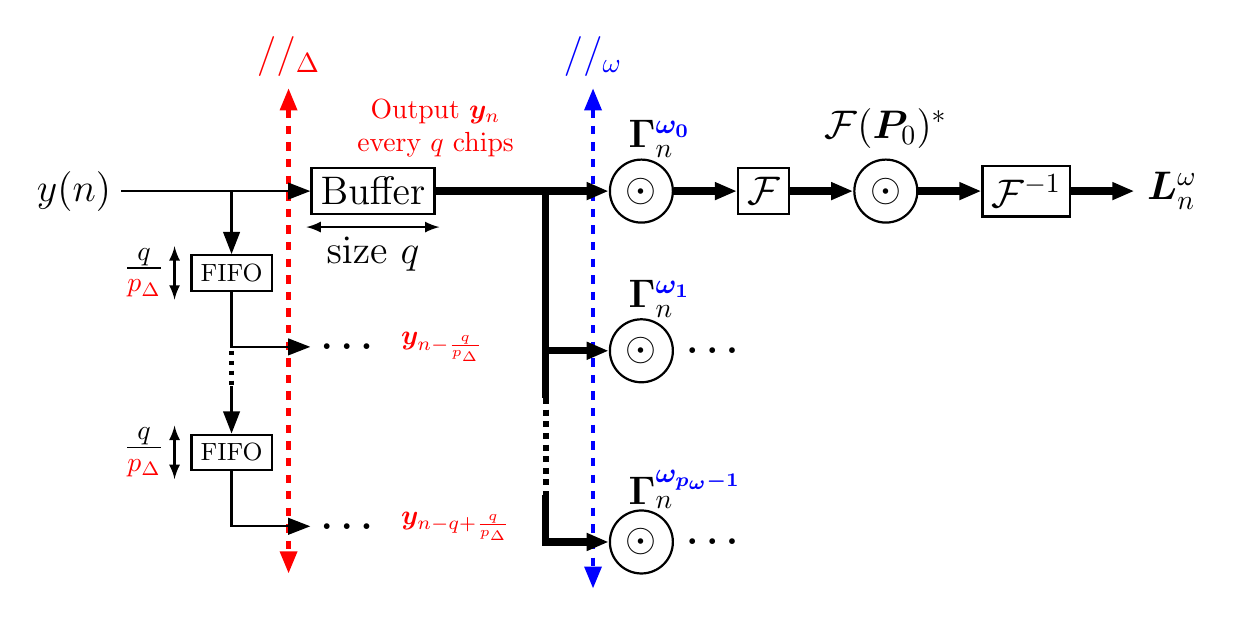
\begin{tikzpicture} [->,
  >={Triangle[width=6pt, length=8pt]},
  auto,
  thick,
  every node/.style={font={\Large}},
  main node/.style={rectangle, fill = white!35, draw,
      align=center}
  ]

  \node [main node,
    draw = none,
    % fill = gray!40!white, 
    % minimum size = 1cm
  ] (input) {$y(n)$};

  \node [main node,
    draw,
    % fill = gray!40!white, 
    % minimum size = 1cm
    right = 2.4 cm of input
  ] (pack) {Buffer};

  \coordinate (ankin) at ($(pack.west) + (-1, 0)$);

  \node [main node,
    anchor = north,
    % fill = gray!40!white, 
    % minimum size = 1cm
  ] (ff1) at ($(ankin) + (0, -.8)$) {\small FIFO};

  \node [main node,
    anchor = north,
    % fill = gray!40!white, 
    % minimum size = 1cm
  ] (ff2) at ($(ff1.south) + (0, -1.8)$) {\small FIFO};

  \node [
    anchor = west,
    % fill = gray!40!white, 
    % minimum size = 1cm
  ] (pack1) at ($(ff1.south east -| pack.west) + (0, -.7)$) {\textbf{\dots}};

  \node [
    anchor = west,
    % fill = gray!40!white, 
    % minimum size = 1cm
  ] (pack2) at ($(ff2.south east -| pack.west) + (0, -.7)$) {\textbf{\dots}};

  \draw [red, dashed, {Triangle[width=6pt, length=8pt]}-{Triangle[width=6pt, length=8pt]}, ultra thick] ($(pack.north west -| ff2.east) + (.2, 1.)$) -- ($(ff2.south east) + (.2, -1.3)$)
  node [anchor = south, pos = 0] (pdelta) {$//_\Delta$};

  \draw (input.east) -> (pack.west);
  \draw [latex-latex] ($(pack.south west) + (-.05, -.15)$) -> ($(pack.south east) + (.05, -.15)$)
  node [midway, anchor = north] {size $q$};

  \draw (ff1.south) |- (pack1.west);
  \draw [latex-latex] ($(ff1.north west) + (-.2, .1)$) -> ($(ff1.south west) + (-.2, -.1)$)
  node [midway, anchor = east] { $\frac{q}{\textcolor{red}{p_\Delta}}$};

  \draw (ff2.south) |- (pack2.west);
  \draw [latex-latex] ($(ff2.north west) + (-.2, .1)$) -> ($(ff2.south west) + (-.2, -.1)$)
  node [midway, anchor = east] { $\frac{q}{\textcolor{red}{p_\Delta}}$};

  \draw (ankin) -> (ff1.north);


  \draw [-] (ff1.south) -> ($(ff1.south) + (0, -.6)$);

  \draw [dotted, -, ultra thick] ($(ff1.south) + (0, -.75)$) -> ($(ff2.north) + (0, .6)$);
  \draw ($(ff2.north) + (0, .6)$) -> (ff2.north);

  \node [circle,
    draw,
    % fill = gray!40!white, 
    right = 2.2 cm of pack,
    minimum size = .8 cm
  ] (multf) {};
  \node [circle,
    draw=none,
    % fill = gray!40!white, 
    anchor = center,
    minimum size = .8 cm
  ] at (multf.center) {\Large $\odot$};
  % \draw [-] ($(multf.north west) + (.1, -.1) $) -- ($(multf.south east) + (-.1,  .1) $);
  % \draw [-] ($(multf.south west) + (.1,  .1) $) -- ($(multf.north east) + (-.1, -.1) $);

  \node [circle,
    draw,
    % fill = gray!40!white, 
    below = 1.2 cm of multf,
    minimum size = .8 cm
  ] (multf1) {};
  \node [circle,
    draw=none,
    % fill = gray!40!white, 
    anchor = center,
    minimum size = .8 cm
  ] at (multf1.center) {\Large $\odot$};
  % \draw [-] ($(multf1.north west) + (.1, -.1) $) -- ($(multf1.south east) + (-.1,  .1) $);
  % \draw [-] ($(multf1.south west) + (.1,  .1) $) -- ($(multf1.north east) + (-.1, -.1) $);
  \node [circle,
    draw=none,
    % fill = gray!40!white, 
    anchor = west,
  ] at (multf1.east) {\textbf{\dots}};

  \node [circle,
    draw,
    % fill = gray!40!white, 
    below = 1.6 cm of multf1,
    minimum size = .8 cm
  ] (multf2) {};
  \node [circle,
    draw=none,
    % fill = gray!40!white, 
    anchor = center,
    minimum size = .8 cm
  ] at (multf2.center) {\Large $\odot$};
  % \draw [-] ($(multf2.north west) + (.1, -.1) $) -- ($(multf2.south east) + (-.1,  .1) $);
  % \draw [-] ($(multf2.south west) + (.1,  .1) $) -- ($(multf2.north east) + (-.1, -.1) $);
  \node [circle,
    draw=none,
    % fill = gray!40!white, 
    anchor = west,
  ] at (multf2.east) {\textbf{\dots}};

  \draw [{Triangle[width=6pt, length=8pt]}-{Triangle[width=6pt, length=8pt]}, ultra thick, blue, dashed] ($(multf.west |- pdelta.south) + (-.2, 0)$) --  ($(multf.west |- multf2.south west) + (-.2, -.3)$)
  node [anchor=south, pos=0] {$//_\omega$};

  % \draw [line width=2.6pt] ($(multf.north) + (0, .5)$) -> (multf.north)
  % node [pos=0, above, align=center] () {$e^{-j\frac{\omega k}{q}}_{(k = 0, 1, \dots, q - 1)}$};
  \node [anchor = south west] at (multf.north west) {$\vect{\Gamma}_{n}^{\bm{\textcolor{blue}{\omega_0}}}$};

  \node [anchor = south west] at (multf1.north west) {$\vect{\Gamma}_{n}^{\bm{\textcolor{blue}{\omega_1}}}$};
  \node [anchor = south west] at (multf2.north west) {$\vect{\Gamma}_{n}^{\bm{\textcolor{blue}{\omega_{p_\omega - 1}}}}$};

  \node [anchor = south east] (ank) at ($(pack.east) + (1.4, 0)$) {};

  \draw [line width=2.6pt] (ank.south east) |- (multf1.west);
  \node [anchor = east] (ank1) at (multf1.west -| ank.east) {};
  \node [anchor = east] (ank2) at (multf2.west -| ank.east) {};

  \draw [line width=2.6pt, -] (ank1.east) -- ($(ank1.east) + (0, -.6)$);
  \draw [line width=2.2pt, -, dotted]  ($(ank1.east) + (0, -.6)$) -- ($(ank2.east) + (0, .6)$);
  \draw [line width=2.6pt] ($(ank2.east) + (0, .6)$) |- (multf2.west);
  % \draw [line width=2.6pt] (ank2.east) |- (multf2.west);

  \node [main node,
    % fill = gray!40!white, 
    % minimum size = 1.2cm,
    right = .8 cm of multf
  ] (fft) {$\mathcal{F}$};

  \draw [line width=2.6pt] (multf.east) -> (fft.west);

  \node [circle,
    draw,
    % fill = gray!40!white,
    right = .8 cm of fft,
    minimum size = .8 cm
  ] (mult) {};
  \node [circle,
    draw=none,
    font={\Large},
    % fill = gray!40!white, 
    anchor = center,
    minimum size = .8 cm
  ] at (mult.center) {$\odot$};
  % \draw [-] ($(mult.north west) + (.1, -.1) $) -- ($(mult.south east) + (-.1,  .1) $);
  % \draw [-] ($(mult.south west) + (.1,  .1) $) -- ($(mult.north east) + (-.1, -.1) $);

  % \draw [line width=2.6pt] ($(mult.north) + (0, .5)$) -> (mult.north)
  % node [pos=0, above, align=center] () {$\mathrm{FFT}(\vect{P}_0)$};
  \node [anchor = south, align=center] () at (mult.north) {$\mathcal{F}(\vect{P}_0)^{\ast}$};

  \draw  [line width=2.6pt] (fft.east) -> (mult.west);

  \node [main node,
    % fill = gray!40!white, 
    % minimum size = 1.2cm,
    right = .8 cm of mult
  ] (ifft) {$\mathcal{F}^{-1}$};

  \draw  [line width=2.6pt] (mult.east) -> (ifft.west);

  % \draw  [line width=2.6pt] ($(multf.west) + (-.8, 0)$) ->  (multf.west)
  % node [pos=0, left, align=center] () {$\vect{y}_n$\\(q chips)};
  \draw  [line width=2.6pt] (pack.east) -> (multf.west);

  \draw  [line width=2.6pt] (ifft.east) -> ($(ifft.east) + (.8, 0)$)
  node [pos=1, right, align=center] () {$\vect{L}_n^\omega$};

  \node [red,
    font = {\normalsize},
    % fill = gray!40!white, 
    % minimum size = 1cm
    anchor = south,
    align = center
  ] at (pack.north east) {Output $\vect{y}_{n}$\\every $q$ chips};

  \node [red,
  font = {\normalsize},
  % fill = gray!40!white, 
  % minimum size = 1cm
  anchor = west,
  align = center
  ] at (pack1.east) {$\vect{y}_{n - \frac{q}{p_{\Delta}}}$};

  \node [red,
  font = {\normalsize},
  % fill = gray!40!white, 
  % minimum size = 1cm
  anchor = west,
  align = center
  ] at (pack2.east) {$\vect{y}_{n - q + \frac{q}{p_{\Delta}}}$};

\end{tikzpicture}

\end{document}
